\chapter*{A Appendix}
\addcontentsline{toc}{chapter}{A Appendix}  
\section*{Code repository}
If you wish to reproduce the results produced from this investigation, I have a GitHub repository which can be found at the following link:

https://github.com/mrehmm001/Deep-Image-Colourisation-comparing-AutoEncoders-and-Conditional-Adversarial-Networks

A dedicated Nvidia GPU is required to enabled GPU accelaration in order to reduce training time. Also, the dataset I've used was from the places365 website which can be found at the followng URL:

http://places2.csail.mit.edu/download.html

Here, I've used "Places-Extra69" version which contains fewer images of 105,000 total. I've partitioned my owned dataset, and if you wish to use mine, here is the URL link:

https://drive.google.com/file/d/178mTebcMLPT5CixUzJOzoDYDLFpVIyNb/view?usp=sharing

I've used author's code to help conduct this research \cite{deepkoal2017code}, \cite{vitoria2020chromagancode}, \cite{vitoria2020chromagancode}.
\pagebreak


\section*{My research}
\begin{figure}[H]
    \centering
    \includegraphics[width=1\columnwidth]{sections/appendix/my_research.JPG}
    \caption{2dsearch was used to help conduct my research}
    \label{fig:my_label}
\end{figure}

\begin{figure}[H]
    \centering
    \includegraphics[width=1\columnwidth]{sections/appendix/my_research_tree.JPG}
    \caption{Literature Research tree diagram}
    \label{fig:my_label}
\end{figure}
\newpage
\chapter*{B Appendix}
\addcontentsline{toc}{chapter}{B Appendix}  

\section*{Neural Networks} 
% \lipsum[1-2]
The Artificial Neural Network (ANN) is a structure that is inspired by the human biological brain, it consists of several processing units (neurons) that have a natural propensity for storing experiential knowledge and making it available for use. As S. Haykin puts it, an ANN resembles the human brain in two respect \cite{haykin2009neural}:
\begin{enumerate}
  \item Knowledge is acquired by the network from its endowment through a learning process. 
  \item interneuron connection strengths, known as synaptic weights, are used to store the acquired knowledge.
\end{enumerate}



\begin{figure}[H]
    \centering
    \includegraphics[width=0.5\columnwidth]{sections/figures/mlp.png}
    \caption{Example of a Artificial Neural Network \cite{mohanty_2019}}
    \label{fig:my_label}
\end{figure}

The learning operation that is used to carry out the action is known as the learning algorithm. The learning algorithm is used during the training phase to modify the synaptic weights of the network. The modification of the synaptic weights will influence the behaviour of the network, which will determine the output of the network.



During the training phase, we have training sets that contain input data with corresponding targets. The input data is fed into the network, and the network performs a process called feedforward. Feedforward involves the summation of synaptic weights and corresponding inputs with the application of activation functions. This results in a predicted output. The predicted output is compared against the actual target output and an error is calculated. This error is used to determine how accurate the network was. If the predicted output is wrong, the network uses a learning algorithm known as the backpropagation algorithm. The backpropagation algorithm computes the gradient descent by calculating the derivative and updating the synaptic weights. This process repeats until the learning algorithm converges into what is known as a global minimum. At the global minimum, learning will cease to proceed. This means the network can classify any input and map it to their corresponding predictions that match the targets.




\subsection{Convolutional Neural Networks}
% \lipsum[1-2]
Convolutional Neural Network (CNN) (also known as convnets) are a special class of ANN used in deep learning and are universally used for computer vision purposes \cite{enwiki:1085146109}. CNN is similar to dense neural networks in ways that CNN consists of input and output layers, as well as several hidden layers, however, the difference lies in the layer: The layer of the CNN consists of a special type of layer called "convolutional layer" (hence the name CNN derives from) that are used to filter out features from the previous layer, called a feature map. The layers also consists of pooling layers which function to reduce the spacial representation size to reduce the number of parameters of the network. The effects of these layers enable CNN to extract complex features from data and learn the representations using fewer parameters, making CNN more efficient at the task of computer vision compared to traditional dense ANN. 

\begin{figure}[H]
    \centering
    \includegraphics[width=0.7\columnwidth]{sections/figures/cnn.JPG}
    \caption{handwriting recognition using CNN \cite{berus_2018}}
    \label{fig:my_label}
\end{figure}



For further information on how Neural Networks word, refer to Haykin's Neural Network textbook \cite{haykin2009neural} amd deep learning with python \cite{franoischollet2017learning}.


\pagebreak
\section*{Tuning results}
The table shown below demonstrates the AutoEncoder tuning results but on a much smaller dataset (Landscapes by blackmamba \cite{landscape}) which contains in total 8,000 images split 60:20:20 ratio. The results are taken from my interim report \cite{mrehm001}. 
\begin{table}[H]
\Huge
\bfseries
\def\arraystretch{2}
\setlength{\tabcolsep}{10pt}
\begin{adjustbox}{width=\textwidth}
\begin{tabular}{|l|l|l|l|l|l|l|}
\hline
Experiments & Optimal epoch & Val loss & Val accuracy & Batch norm & Augmentation & Learning rate \\ \hline
Experiment 1 & 27 & 0.0096 & 0.6548 & No  & No  & Default (1e-3) \\ \hline
Experiment 2 & 14 & 0.0075 & 0.7155 & No  & No  & 1e-4           \\ \hline
Experiment 3 & 21 & 0.0075 & 0.7065 & No  & No  & 1e-5           \\ \hline
Experiment 4 & 85 & 0.0073 & 0.7106 & Yes & Yes & 1e-4           \\ \hline
Experiment 5 & 62 & 0.0071 & 0.7177 & No  & Yes & 1e-4           \\ \hline
\end{tabular}

\end{adjustbox}
\caption{Experiments gathered throughout the training of the model}
\end{table}

\begin{figure}[H]
    \centering
    \includegraphics[width=0.7\columnwidth]{sections/figures/Experiment1.png}
    \caption{Experiment 1 plot}
    \label{fig:my_label}
\end{figure}

\begin{figure}[H]
    \centering
    \includegraphics[width=0.7\columnwidth]{sections/figures/Experiment2.png}
    \caption{Experiment 2 plot}
    \label{fig:my_label}
\end{figure}

\begin{figure}[H]
    \centering
    \includegraphics[width=0.7\columnwidth]{sections/figures/Experiment3.png}
    \caption{Experiment 3 plot}
    \label{fig:my_label}
\end{figure}

\begin{figure}[H]
    \centering
    \includegraphics[width=0.7\columnwidth]{sections/figures/Experiment4.png}
    \caption{Experiment 4 plot}
    \label{fig:my_label}
\end{figure}

\begin{figure}[H]
    \centering
    \includegraphics[width=0.7\columnwidth]{sections/figures/Experiment5.png}
    \caption{Experiment 5 plot}
    \label{fig:my_label}
\end{figure}

\subsection*{Optimal model analysis}
\begin{figure}[H]
    \centering
    \includegraphics[width=1\columnwidth]{sections/figures/optimal.png}
    \caption{Validation and accuracy plots of the optimal model}
    \label{fig:my_label}
\end{figure}

\section*{Training the Pix2Pix using a smaller dataset}
\begin{figure}[H]
    \centering
    \includegraphics[width=1\columnwidth]{sections/figures/pix2pix_training.JPG}
    \caption{Using a smaller dataset (landscape by black mamba \cite{landscape}), the Pix2Pix was trained over 400 epochs over the course of 24 hours. }
    \label{fig:my_label}
\end{figure}

\section*{User study results}
\begin{figure}[H]
    \centering
    \includegraphics[width=1\columnwidth]{sections/appendix/study_result_part1.png}
    \caption{Full user naturalness study results}
    \label{fig:my_label}
\end{figure}

\begin{figure}[H]
    \centering
    \includegraphics[width=1\columnwidth]{sections/appendix/study_result_part2.png}
    \caption{Full user naturalness study results}
    \label{fig:my_label}
\end{figure}

\begin{figure}[H]
    \centering
    \includegraphics[width=1\columnwidth]{sections/appendix/study_result_part3.png}
    \caption{Full user naturalness study results}
    \label{fig:my_label}
\end{figure}

\begin{figure}[H]
    \centering
    \includegraphics[width=1\columnwidth]{sections/appendix/study_result_part4.png}
    \caption{Full user naturalness study results}
    \label{fig:my_label}
\end{figure}

% \section*{More colourisation showcase}
% \begin{figure}[H]
%     \centering
%     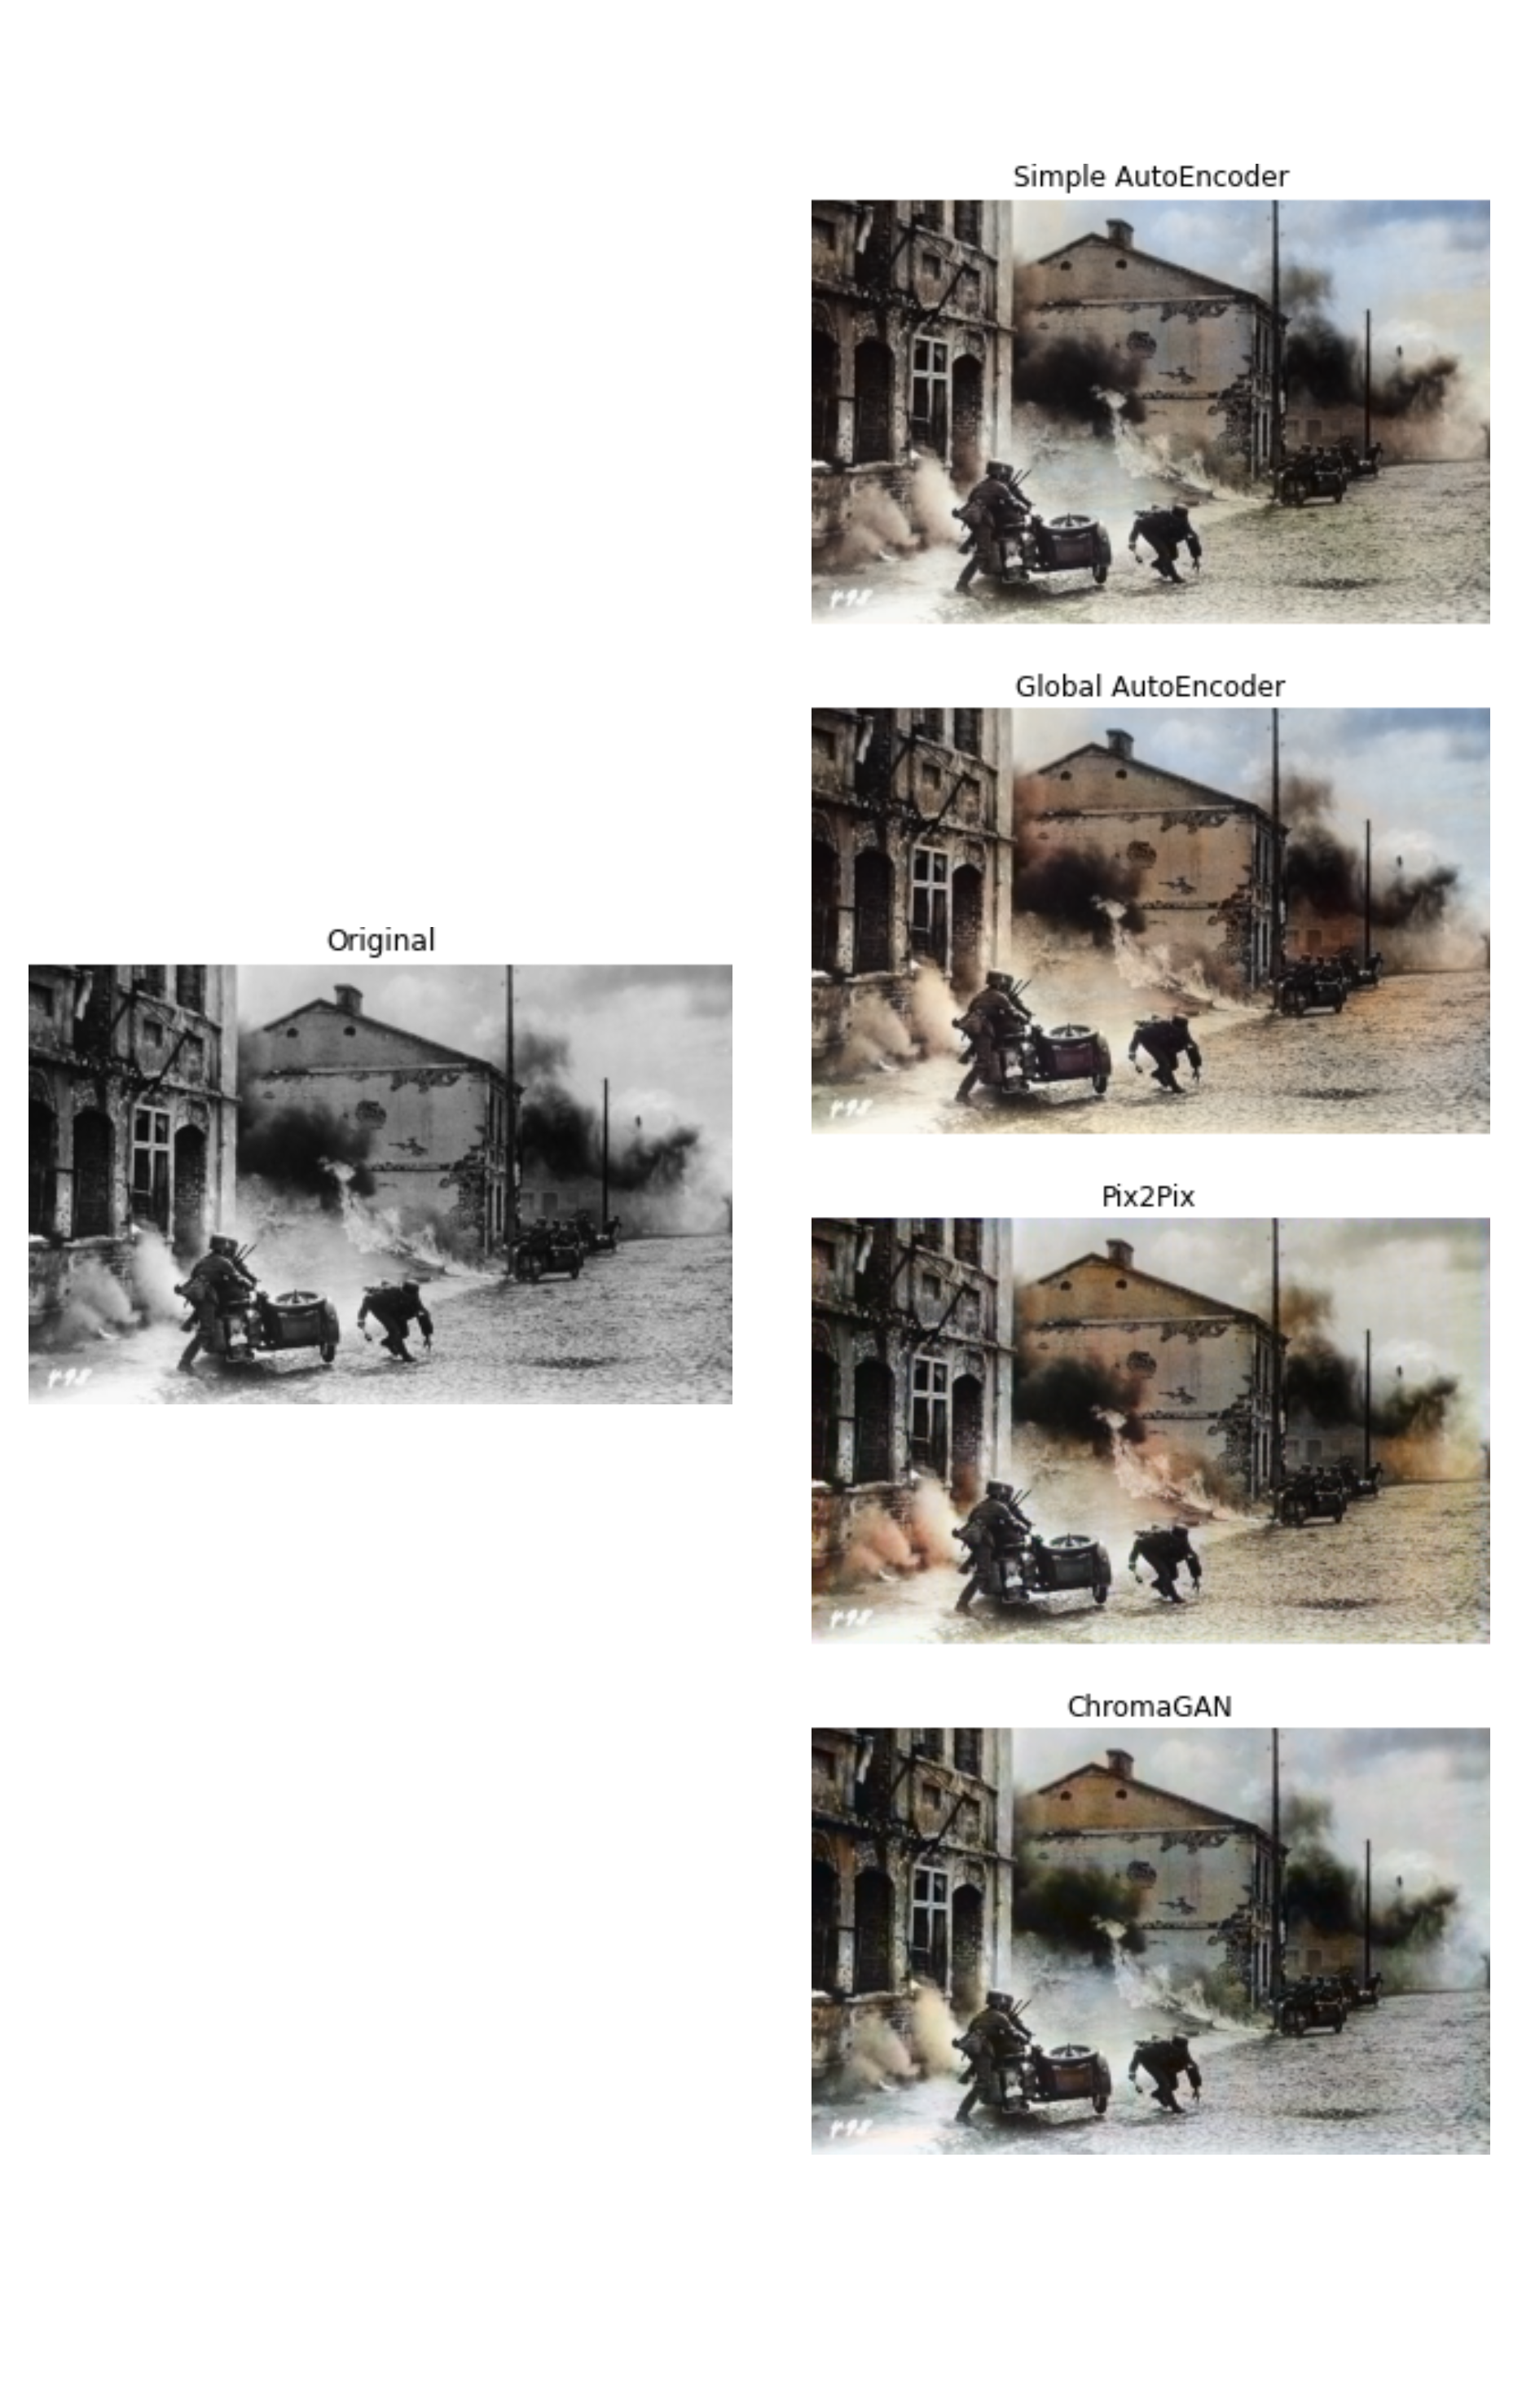
\includegraphics[width=1\columnwidth]{sections/appendix/result_1.png}
%     \caption{Colourisation results}
%     \label{fig:my_label}
% \end{figure}

% \begin{figure}[H]
%     \centering
%     \includegraphics[width=1.1\columnwidth]{sections/appendix/result_2.png}
%     \caption{Colourisation results}
%     \label{fig:my_label}
% \end{figure}
% \begin{figure}[H]
%     \centering
%     \includegraphics[width=1.1\columnwidth]{sections/appendix/result_3.png}
%     \caption{Colourisation results}
%     \label{fig:my_label}
% \end{figure}
% \begin{figure}[H]
%     \centering
%     \includegraphics[width=1.05\columnwidth]{sections/appendix/result_4.png}
%     \caption{Colourisation results}
%     \label{fig:my_label}
% \end{figure}
% \begin{figure}[H]
%     \centering
%     \includegraphics[width=1\columnwidth]{sections/appendix/result_5.png}
%     \caption{Colourisation results}
%     \label{fig:my_label}
% \end{figure}
% \begin{figure}[H]
%     \centering
%     \includegraphics[width=1\columnwidth]{sections/appendix/result_6.png}
%     \caption{Colourisation results}
%     \label{fig:my_label}
% \end{figure}



\chapter*{C Appendix}
\addcontentsline{toc}{chapter}{C Appendix}  
\section*{Video colourisation results}
I have carried out colourisation of historical footages to see how they'd perform.


\begin{figure}[H]
    \centering
    \includegraphics[width=1\columnwidth]{sections/appendix/ww2_colourisation1.JPG}
    \caption{WW2 combat footage colourised using Simple AutoEncoder. Link: https://youtu.be/OW9Sdq4ejSo}
    \label{fig:my_label}
\end{figure}


\begin{figure}[H]
    \centering
    \includegraphics[width=1\columnwidth]{sections/appendix/ww2_colourisation2.JPG}
    \caption{WW2 combat footage colourised using Global AutoEncoder. Link: https://youtu.be/J4YZ3RDdiig}
    \label{fig:my_label}
\end{figure}


\begin{figure}[H]
    \centering
    \includegraphics[width=1\columnwidth]{sections/appendix/ww2_colourisation3.JPG}
    \caption{WW2 combat footage colourised using Pix2Pix. Link: https://youtu.be/fuUdiurJ_qI}
    \label{fig:my_label}
\end{figure}

\begin{figure}[H]
    \centering
    \includegraphics[width=1\columnwidth]{sections/appendix/ww2_colourisation4.JPG}
    \caption{WW2 combat footage colourised using ChromaGAN. Link: https://youtu.be/jiF394SHxI4}
    \label{fig:my_label}
\end{figure}


\begin{figure}[H]
    \centering
    \includegraphics[width=1\columnwidth]{sections/appendix/new_york_colourisation.JPG}
    \caption{Black and white footage of new york ChromaGAN. Link:  https://youtu.be/nqlh5KMAf3I | original footage link: https://www.youtube.com/watch?v=f-d88HkWFtQ}
    \label{fig:my_label}
\end{figure}